\chapter{Deadlock}s a Resource Allocation
Graph?}\label{what-is-a-resource-allocation-graph}

A resource allocation graph tracks which resource is held by which
process and which process is waiting for a resource of a particular
type. It is very powerful and simple tool to illustrate how interacting
processes can deadlock.

If there is a cycle in the Resource Allocation Graph then the processes
will deadlock. For example, if process 1 holds resource A, process 2
holds resource B and process 1 is waiting for B and process 2 is waiting
for A, then process 1 and 2 process will be deadlocked.

Here's another example, that shows Processes 1 and 2 acquiring resources
1 and 2 while process 3 is waiting to acquire both resources. In this
example there is no deadlock because there is no circular dependency.

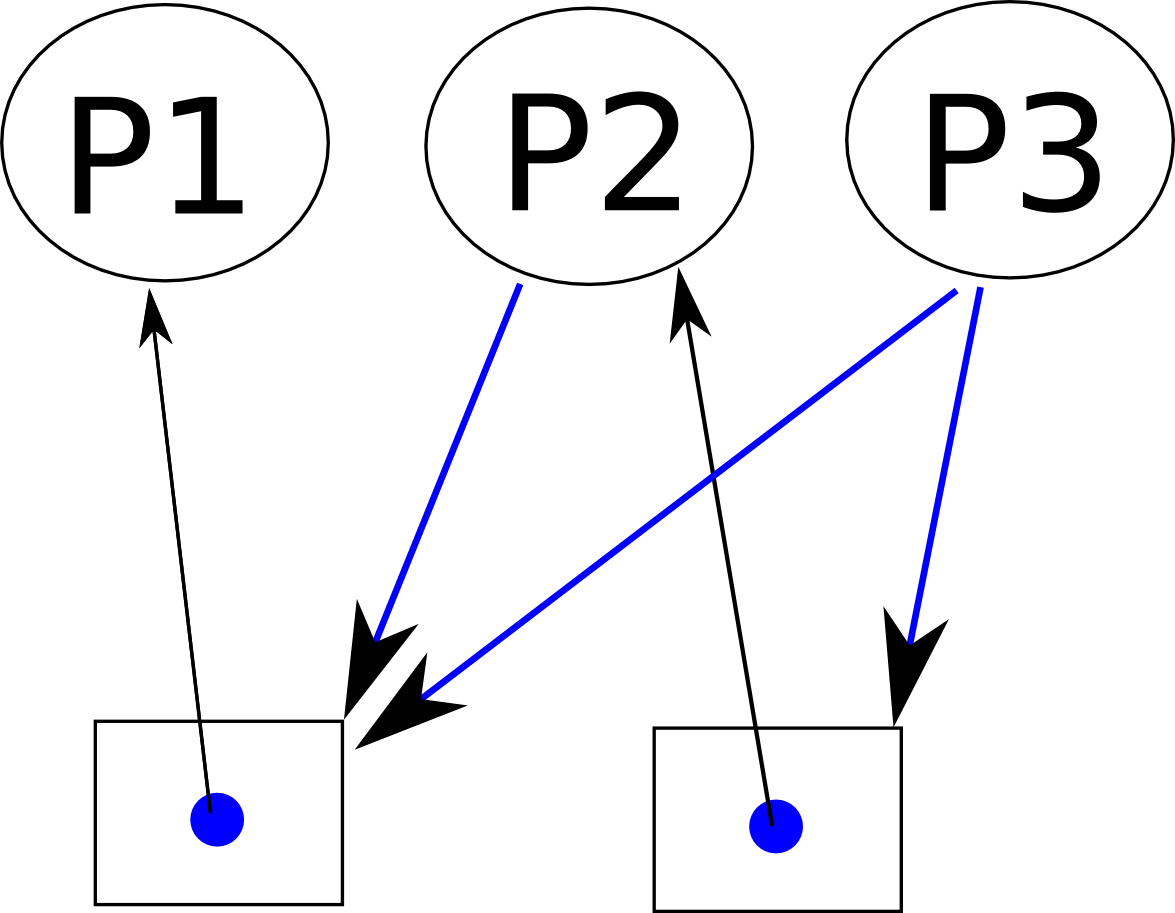
\includegraphics{https://raw.githubusercontent.com/wiki/angrave/SystemProgramming/ResourceAllocationGraph-Ex1.png}

Todo: More complicated example
